\documentclass{article}

% packages
  % basic stuff for rendering math
  \usepackage[letterpaper, top=1in, bottom=1in, left=1in, right=1in]{geometry}
  \usepackage[utf8]{inputenc}
  \usepackage[english]{babel}
  \usepackage{amsmath} 
  \usepackage{amssymb}
  % \usepackage{amsthm}

  % extra math symbols and utilities
  \usepackage{mathtools}        % for extra stuff like \coloneqq
  \usepackage{mathrsfs}         % for extra stuff like \mathsrc{}
  \usepackage{centernot}        % for the centernot arrow 
  \usepackage{bm}               % for better boldsymbol/mathbf 
  \usepackage{enumitem}         % better control over enumerate, itemize
  \usepackage{hyperref}         % for hypertext linking
  \usepackage{fancyvrb}          % for better verbatim environments
  \usepackage{newverbs}         % for texttt{}
  \usepackage{xcolor}           % for colored text 
  \usepackage{listings}         % to include code
  \usepackage{lstautogobble}    % helper package for code
  \usepackage{parcolumns}       % for side by side columns for two column code
  

  % page layout
  \usepackage{fancyhdr}         % for headers and footers 
  \usepackage{lastpage}         % to include last page number in footer 
  \usepackage{parskip}          % for no indentation and space between paragraphs    
  \usepackage[T1]{fontenc}      % to include \textbackslash
  \usepackage{footnote}
  \usepackage{etoolbox}

  % for custom environments
  \usepackage{tcolorbox}        % for better colored boxes in custom environments
  \tcbuselibrary{breakable}     % to allow tcolorboxes to break across pages

  % figures
  \usepackage{pgfplots}
  \pgfplotsset{compat=1.18}
  \usepackage{float}            % for [H] figure placement
  \usepackage{tikz}
  \usepackage{tikz-cd}
  \usepackage{circuitikz}
  \usetikzlibrary{arrows}
  \usetikzlibrary{positioning}
  \usetikzlibrary{calc}
  \usepackage{graphicx}
  \usepackage{caption} 
  \usepackage{subcaption}
  \captionsetup{font=small}

  % for tabular stuff 
  \usepackage{dcolumn}

  \usepackage[nottoc]{tocbibind}
  \pdfsuppresswarningpagegroup=1
  \hfuzz=5.002pt                % ignore overfull hbox badness warnings below this limit

% New and replaced operators
  \DeclareMathOperator{\Tr}{Tr}
  \DeclareMathOperator{\Sym}{Sym}
  \DeclareMathOperator{\Span}{span}
  \DeclareMathOperator{\std}{std}
  \DeclareMathOperator{\Cov}{Cov}
  \DeclareMathOperator{\Var}{Var}
  \DeclareMathOperator{\Corr}{Corr}
  \DeclareMathOperator{\pos}{pos}
  \DeclareMathOperator*{\argmin}{\arg\!\min}
  \DeclareMathOperator*{\argmax}{\arg\!\max}
  \newcommand{\ket}[1]{\ensuremath{\left|#1\right\rangle}}
  \newcommand{\bra}[1]{\ensuremath{\left\langle#1\right|}}
  \newcommand{\braket}[2]{\langle #1 | #2 \rangle}
  \newcommand{\qed}{\hfill$\blacksquare$}     % I like QED squares to be black

% Custom Environments
  \newtcolorbox[auto counter, number within=section]{example}[1][]
  {
    colframe = orange!25,
    colback  = orange!10,
    coltitle = orange!20!black,  
    breakable, 
    title = \textbf{Question \thetcbcounter ~(#1)}
  }
  \newtcolorbox[auto counter, number within=section]{definition}[1][]
  {
    colframe = yellow!25,
    colback  = yellow!10,
    coltitle = yellow!20!black,  
    breakable, 
    title = \textbf{Definition \thetcbcounter ~(#1)}
  } 
  \newtcolorbox[auto counter, number within=section]{society}[1][]
  {
    colframe = teal!25,
    colback  = teal!10,
    coltitle = teal!20!black,  
    breakable, 
    title = \textbf{Society \thetcbcounter}
  }
  \newtcolorbox[auto counter, number within=section]{politics}[1][]
  {
    colframe = red!25,
    colback  = red!10,
    coltitle = red!20!black,  
    breakable, 
    title = \textbf{Politics \thetcbcounter ~(#1)}
  }
  \newtcolorbox[auto counter, number within=section]{legal}[1][]
  {
    colframe = blue!25,
    colback  = blue!10,
    coltitle = blue!20!black,  
    breakable, 
    title = \textbf{Legal \thetcbcounter ~(#1)}
  } 
  \newtcolorbox[auto counter, number within=section]{finance}[1][]
  {
    colframe = green!25,
    colback  = green!10,
    coltitle = green!20!black,  
    breakable, 
    title = \textbf{Finance \thetcbcounter ~(#1)}
  } 
  \newtcolorbox[auto counter, number within=section]{religion}[1][]
  {
    colframe = violet!25,
    colback  = violet!10,
    coltitle = violet!20!black,  
    breakable, 
    title = \textbf{Religion \thetcbcounter ~(#1)}
  }

  \BeforeBeginEnvironment{example}{\savenotes}
  \AfterEndEnvironment{example}{\spewnotes}
  \BeforeBeginEnvironment{lemma}{\savenotes}
  \AfterEndEnvironment{lemma}{\spewnotes}
  \BeforeBeginEnvironment{theorem}{\savenotes}
  \AfterEndEnvironment{theorem}{\spewnotes}
  \BeforeBeginEnvironment{corollary}{\savenotes}
  \AfterEndEnvironment{corollary}{\spewnotes}
  \BeforeBeginEnvironment{proposition}{\savenotes}
  \AfterEndEnvironment{proposition}{\spewnotes}
  \BeforeBeginEnvironment{definition}{\savenotes}
  \AfterEndEnvironment{definition}{\spewnotes}
  \BeforeBeginEnvironment{exercise}{\savenotes}
  \AfterEndEnvironment{exercise}{\spewnotes}
  \BeforeBeginEnvironment{proof}{\savenotes}
  \AfterEndEnvironment{proof}{\spewnotes}
  \BeforeBeginEnvironment{solution}{\savenotes}
  \AfterEndEnvironment{solution}{\spewnotes}
  \BeforeBeginEnvironment{question}{\savenotes}
  \AfterEndEnvironment{question}{\spewnotes}
  \BeforeBeginEnvironment{code}{\savenotes}
  \AfterEndEnvironment{code}{\spewnotes}

  \definecolor{dkgreen}{rgb}{0,0.6,0}
  \definecolor{gray}{rgb}{0.5,0.5,0.5}
  \definecolor{mauve}{rgb}{0.58,0,0.82}
  \definecolor{lightgray}{gray}{0.93}

  % default options for listings (for code)
  \lstset{
    autogobble,
    frame=ltbr,
    language=C,                           % the language of the code
    aboveskip=3mm,
    belowskip=3mm,
    showstringspaces=false,
    columns=fullflexible,
    keepspaces=true,
    basicstyle={\small\ttfamily},
    numbers=left,
    firstnumber=1,                        % start line number at 1
    numberstyle=\tiny\color{gray},
    keywordstyle=\color{blue},
    commentstyle=\color{dkgreen},
    stringstyle=\color{mauve},
    backgroundcolor=\color{lightgray}, 
    breaklines=true,                      % break lines
    breakatwhitespace=true,
    tabsize=3, 
    xleftmargin=2em, 
    framexleftmargin=1.5em, 
    stepnumber=1
  }

% Page style
  \pagestyle{fancy}
  \fancyhead[L]{Fertile Crescent}
  \fancyhead[C]{Muchang Bahng}
  \fancyhead[R]{Spring 2024} 
  \fancyfoot[C]{\thepage / \pageref{LastPage}}
  \renewcommand{\footrulewidth}{0.4pt}          % the footer line should be 0.4pt wide
  \renewcommand{\thispagestyle}[1]{}  % needed to include headers in title page

\begin{document}

\title{Civilizations in the Fertile Crescent}
\author{Muchang Bahng}
\date{Spring 2024}

\maketitle
\tableofcontents
\pagebreak

  In here I talk about the development of two of the cradles of civilization: the Mesopotamians and Egyptians. I conglomorated them into a single set of notes since they were quite interdependent and were physically the same. We start off with the civilizations in the \textbf{Fertile Crescent}, which is shown below. 

  \begin{figure}[H]
    \centering 
    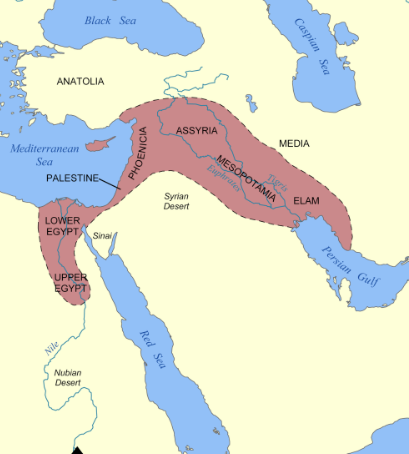
\includegraphics[scale=0.4]{img/fertile_crescent.png}
    \caption{The Fertile Crescent is a crescent-shaped region in the Middle East, spanning modern-day Iraq, Syria, Lebanon. As we will see later, the advance of agriculture made this region a great place to settle. } 
    \label{fig:fertile_crescent}
  \end{figure}

  But to talk about civilizations, we must first define what it is and differentiate it from other forms of human organization like hunter gatherers, tribes, or cavemen. The rigorous definition is often debated, so we will stick with the following rudimentary one. 

  \begin{definition}[Civilization]
    A \textbf{civilization} is a complex society characterized by the following 
    \begin{enumerate}
      \item \textbf{Urban development} is the process of creating cities. 
      \item \textbf{Social stratification} is the division of society into classes. 
      \item A form of \textbf{government} is the system by which a state or community is controlled. 
      \item \textbf{Symbolic communication forms} like writing.
    \end{enumerate}
  \end{definition}

  A more rudimentary version of civilization is called a \textbf{culture}. 

  \begin{definition}[General Timeline]
    The following is general taxonomy of human history. 
    \begin{enumerate} 
      \item (-3000 BCE) The \textbf{Stone age} is a prehistoric period during which stone was widely used to make stone tools, lasting for approximately 3.4 million years. It is divided into 3 subcategories. 
        \begin{enumerate}
          \item (- 9000 BCE) The \textbf{Paleolithic era} is the primitive use of stones. 
          \item The \textbf{Mesolithic era} is transitionary period. 
          \item (9000 - 3000 BCE) The \textbf{Neolithic era} is the final stage characterized by agriculture. 
        \end{enumerate}
      \item (3000 - 1200 BCE) The \textbf{Bronze age} is characterized by the use of bronze tools, the use of writing in some areas, and the features of urban civilization. 
      \item (1200 - 550 BCE) The \textbf{Iron age} evolved from bronze to iron. 
    \end{enumerate}
  \end{definition}

\section{Pre-Sumerian Hunter Gatherers}

  \subsection{Hunter Gatherers}

    The \textbf{Stone Age} is a prehistoric period during which stone was widely used to make stone tools, lasting for approximately 3.4 million years.\footnote{The period of time before civilization developed is called \textbf{prehistory}. } The majority of the Stone age was spent in the \textbf{Paleolithic era}, where humans were hunter gatherers, which were bands of humans, often an extended family but growing up to 100 people, who traveled around for food and shelter. Guided by their knowledge in geography, each group would travel across a span of land hundreds of miles wide, following the migration of animals, the growth of plants, and the changing of seasons. 

    Note that this was inherently limited. First, with a limited supply of food in each area, groups cannot be unbounded in size. Larger groups meant more traveling, and at some point you would have to travel at an unsustainable pace, which is why there was an inherent limit in these sizes. 

    Even at this rudimentary stage, there was some specialization of labor, with the first example being that males, who were physically stronger, would hunt, and females would gather vegetation and take care of children. This allowed for a more efficient use of resources. With individuals specializing in their tasks, one would think that \textbf{bartering}, the practice of trading good and services, would have been common. However, there is not much evidence for this. Rather, one a group had secured a resource, it would simply be distributed within the tribe. 

    Furthermore, there was no social stratification, as everyone was equal. There may have been leaders who directed the group, but they were not considered superior to others. Similarly, there was no concept of private property. 

    Interactions between two tribes are not well known, and it is hard to tell how territorial they may have been. The main reason would have been for a competition of resources, but these communities may have traveled rotationally so that they don't bump into each other. 

  \subsection{Neolithic Era}

    However, around 9000 BCE, the \textbf{Neolithic era} began, where various hunter gatherers began to separate from their main groups and begin settlements, staring with those in the Fertile Crescent and others following rapidly. This had several consequences. 

    \begin{society}[Population Growth]
      There was an explosive population growth. Since they were not limited by the ability to travel and were self-sustaining, they could feed more mouths and often had a surplus of food. 
    \end{society}

    \begin{finance}[Private Property]
      With settlements, households began to own private property by building their own shelters (with adobe) on claimed land. More sophisticated tools like clay pottery were also developed. 
    \end{finance}

    \begin{finance}[Social Inequality]
      The domestication and possession of large animals resulted in a dramatic increase in social inequality since it allowed competition between households and resulted in inherited inequalities of wealth. This led to tribal leaders, chiefs, or small elite groups of people (though this was not pronounced until the Bronze age).\footnote{This would be the birth of primitive governments.} 
    \end{finance}

    \begin{finance}[Sophsitication of Bartering]
      With households working in each area of labor, the surplus of grain and cattle allowed more sophisticated forms of bartering, though a common currency was not established yet and values can still be negotiated. 
    \end{finance}

    \begin{finance}[First Bookkeeping Practices]
      Bookkeeping of agricultural production was established. At this point writing may not have been invented yet, and so farmers would take clay tokens and store them in pots as a method of accounting. This gave rise to the first accounting practices in humanity that tracked whether surplus had been gained. 
    \end{finance}

    Over the next millennia, these settlements would grow at this pace to become city-states, and Mesopotamia would be scattered with independent city-states in this \textit{Chalcolithic period}. Major city-states, whose names will become important, were Uruk, Ur, Kish and Eridu. 

\section{Sumerians}

  Around 3500 BCE, the ancient \textbf{Sumerians} (whose origin is not well known but was believed to have migrated) settled into the city of Uruk Mesopotamia near the Tigris and Euphrates rivers, giving rise to the \textbf{Uruk period}. 

  \begin{finance}[Writing]
    To more effectively practice accounting, the Sumerians learned that imprinting symbols on wet clay tablets was much easier and accurate, giving birth to the \textbf{Cuneiform writing} system. It would be used for the next 3 millennia. 
  \end{finance}

  \subsection{The First Banks}

    \begin{religion}[Agricultural Gods]
      At this point Uruk would hold tens of thousands of inhabitants, and to support this massive population they depended heavily on agriculture. Mesopotamia's climate was prone to floods and had extremely hot summers, making agriculture risky at times. The citizens' understanding of these changing climate was that it was controlled by a God. To please this God, they worshipped it with temples, known as \textbf{ziggurats}, placed in the center of cities. In here, they would pay tributes and offer sacrifices to please the God and receive good weather. 
    \end{religion}
    
    Therefore, a typical city would consist of an elevated ziggurat in the center, surrounded by living quarters for the citizens, surrounded by a wall.\footnote{From previous experiences in warfare with neighboring city-states, these cities would first have walls. } Beyond the walls, there would be a massive stretch of farmland with irrigation channels that supported the population.

    A typical farming season would consist of farmers resting in cities for the summer, and when the weather got cooler, they would go out to repair irrigation channels, plant seeds, and finally harvest their crops. These methods were extremely effective and produced bountiful surplus, which were needed to plant next year's crops, use a livestock feed, or for human consumption. 

    The problem was storing it, since if you store it in the farmer's houses they can be flooded, resulting in the seeds sprouting too early. Therefore, much of these grains were stored in the elevated ziggurats, and so when it came time to harvest, farmers would go out, get the crops, and carry them back to the ziggurats. But this leads to another problem. From the perspective of a farmer who bothered to transport all that grain, I would want to ensure that I can be the one who eats it or at least in possession of it. 

    One way to do this was use some form of currency like clay coins. You, as a farmer, can take your grains to a temple and exchange the grain for coins. Later on, you can come back to the temple and buy back the grain. This gave birth to the first banking system in civilization, but there was one problem. It was extremely easy to counterfeit these coins, since they're just little balls of hardened clay. This was solved by using envelopes. 

    \begin{finance}[Temples as the First Banks]
      To combat this, the Sumerians had clay ``envelopes.'' Say that one coin is worth 1 pound of barley, and you want to store 10 pounds in the temple. Rather than just receiving 10 coins. You would do the following. 
      \begin{enumerate}
        \item You take the 10 pounds to the temple and meet the priest there. 
        \item The priest mints 10 coins for you and 10 coins for him. He then puts 10 coins in one hardened clay ball envelop and 10 coins in the other.  
        \item Then, he marks that there were 10 coins the outside of the envelope, hardens the envelope, and gives it back to you. 
      \end{enumerate}
      At this point, you have an envelope to take back home and the priest has one kept in the temple. Given that you don't break the envelope, you can take it back to the temple at a future time, where both you can the priest can first take a look at the inscriptions to see that they match, then break open the envelopes to see that the coins inside match, and then you receive your 10 pounds of grain. This is essentially a deposit and can't be counterfeited.\footnote{There are obvious disadvantages to this system, but it was good enough to work. } 
    \end{finance} 

  \subsection{Silver and Barley as Currency}

    We can understand now that the origin of banks comes from a need to safely store grains, mainly barley, and so barley is by many considered to be the first official currency of the world. Before, we move on, though, we should probably define what money can or can not be. Again, the definition is still debated today, so will use the following rudimentary one.

    \begin{definition}[Money]
      There are four criteria to determine whether something is judged as money. 
      \begin{enumerate}
        \item It can be used as a means of payment.\footnote{You can give a slab of meat for berries. } 
        \item It can be used as a medium to facilitate indirect exchange, i.e. exchanging object A for money, and money for object B. 
        \item It can serve as a standard of value. 
        \item It can be served as a means of storing wealth. 
      \end{enumerate}
    \end{definition}

    Another common type in Sumerian society was silver.\footnote{It's not quite certain how Sumerians had access to silver since precious metals were hard to find in Mesopotamia. It may have been through trade with neighboring civilizations. It is also not sure how the absolute value of silver was set as well. }, which has its own denominations. 

    \begin{definition}[Denominations of Grain] 
      Barley and wheat were common forms of grain. A \textbf{sila} is about 1 liter. A \textbf{kur} is about 180 kilograms, or 30 silas.
    \end{definition}

    \begin{definition}[Denominations of Silver]
      For this context, we only need to know that a \textbf{shekel}, or \textbf{gin}, of silver is about 3 pennies weight. It has the following value 
      \begin{enumerate}
        \item it can buy about 30 silas of wheat/barley, which is almost a year's worth for one person. 
        \item 10 to 20 shekels can buy about 1 slave. 
      \end{enumerate}
      A \textbf{mina} was 60\footnote{They used base 60 numbers.} shekels and \textbf{talent} was 60 minas. 
    \end{definition}

    There were other forms of money through different commodities, but they weren't used as much as a \textit{standard} per se. 

  \subsection{Loans and Debt}

    At this point, the concept of loans took off as well.
    
    \begin{finance}[Loans and Interests in Sumer]
      Mainly between the elite and institutions, those with surplus could lend their resources to others. This can happen between royalty, individuals, or the temple, leading to improved \textbf{liquidity} of money. The more efficient flow of money from those who have excess to those in need also increased productivity. These loans would be written in tablets that described 
      \begin{enumerate}
        \item the parties involved 
        \item the quantity of the commodity loaned 
        \item when it will be paid back and consequences for not paying
        \item interest rates, which were explicitly put as a percentage or quantity of the loaned commodity, or if omitted, was presumed to be common knowledge.\footnote{For cattle, which was often traded, the interest would be any offspring that they produced. }\footnote{Before Sumer, loaning at interest did not seem to exist. }
      \end{enumerate}
    \end{finance}

    \begin{example}[Loan]
      The following is an example of a loan between two high-class members, with collateral being barley. There is a hefty fee for not returning the silver (2 gur, or 600 silas, or barley per shekel of silver, when one shekel buys 30 silas.)

      \begin{center}
        “Su-asli received 25 gin of silver from Azida. He will return the silver in its entirety in month 8 in Nippur. If he does not return it, he will weigh out 2 gur of barley for each shekel of silver after the harvest. …”
      \end{center}
    \end{example}

    Sometimes, during special occasions, kings would cancel debts. 

  \subsection{Taxation} 

    \begin{definition}[Taxes]
      While there were instances of it in Mesopotamia, the Egyptians at this time had invented taxation. 
    \end{definition}


  \subsection{Early Dynastic Period}

    This is all within one city-state. There were rivals, so inter-city-state trade was not allowed at this point. 

    Enshakushanna of Uruk conquered all of Sumer, Akkad, and Hamazi, followed by Eannatum of Lagash who also conquered Sumer. His methods were force and intimidation (see the Stele of the Vultures), and soon after his death, the cities rebelled and the empire again fell apart. Some time later, Lugal-Anne-Mundu of Adab created the first, if short-lived, empire to extend west of Mesopotamia, at least according to historical accounts dated centuries later. The last native Sumerian to rule over most of Sumer before Sargon of Akkad established supremacy was Lugal-Zage-Si. 

    With the development of power, there were inevitably conflicts between the Sumerian city-states such as Kish, Uruk, Ur, and Lagash. The details aren't relevant, but Sumerians remained a bunch of warring city states until \textit{Sargon of Akkad}. 


\section{Akkadian Empire and the Ur III Period}

  Then, \textit{Sargon of Akkad} had established himself as ruler in 2350 BCE. 

\section{Assyrian Empire}



\section{Babylonian Empire}

  Hammurabi. 

\end{document}
